\documentclass[14pt, oneside]{altsu-bachelor}

\title{Сервис автоматизированного решения CAPTCHA}
\author{А.\,В.~Лаптев}
\groupnumber{5.306M}
\GradebookNumber{1337}
\supervisor{В.\,В.~Электроник}
\supervisordegree{к.ф.-м.н., доцент}
\ministry{Министерство науки и высшего образования}
\country{Российской Федерации}
\fulluniversityname{ФГБОУ ВО Алтайский государственный университет}
\institute{Институт цифровых технологий, электроники и физики}
\department{Кафедра вычислительной техники и электроники}
\departmentchief{В.\,В.~Пашнев}
\departmentchiefdegree{к.ф.-м.н., доцент}
\shortdepartment{ВТиЭ}
\ChairmanOfTheStateCertificationCommission{С.\,П.~Пронин}
\ChairmanOfTheStateCertificationCommissiondegree{д.т.н., проф.}
\NormController{А.\,В.~Калачёв}
\NormControllerdegree{к.ф.-м.н., доцент}
\Consultant{}
\Consultantdegree{}
\UDC{004.94}
\docname{БР 09.03.01}
\abstractRU{Объём текста не менее 1000 символов! Пока счётчики выставляются в ручную, при необходимости правьте cls-файл.}
\abstractEN{Большой текст на английском!}
\keysRU{компьютерное моделирование, cистема управления версиями}
\keysEN{computer simulation, distributed version control}
\countWorkPage{22}
\countWorkImg{6}
\countWorkLit{5}
\countWorkTab{6}

\date{\the\year}

% Подключение файлов с библиотекой.
\addbibresource{graduate-students.bib}

\begin{document}
\maketitle

\setcounter{page}{2}
\makeabstract
\tableofcontents

\chapter{Теоретические основы и эволюция технологии CAPTCHA}

\section{Происхождение и функциональное назначение CAPTCHA}

Проверочный код CAPTCHA (Completely Automated Public Turing test to tell Computers 
and Humans Apart) -- это метод защиты, основанный на принципе аутентификации 
<<вызов-ответ>>. Он предназначен для предотвращения автоматических действий, таких 
как спам или попытки взлома учетных записей, путем выполнения пользователем 
простого теста, подтверждающего, что он человек, а не программа~\cite{support}. 
Термин был придуман в 2003 году~\cite{captcha2003}.

Исторически распространенный тип CAPTCHA был впервые изобретен в 1997 году двумя 
группами, работающими параллельно. Эта форма CAPTCHA требует ввода 
последовательности букв или цифр из искаженного изображения. Поскольку тест 
проводится компьютером, в отличие от стандартного теста Тьюринга, который 
проводится человеком, CAPTCHA иногда описываются как обратные тесты Тьюринга
~\cite{reversecaptcha}.

Набравшая популярность технология reCAPTCHA, была приобретена Google в 2009 году
~\cite{googlerecaptcha}. В дополнение к предотвращению мошенничества с ботами для 
пользователей, Google использовал технологию reCAPTCHA для оцифровки архивов The 
New York Times и книг из Google Books в 2011 году~\cite{nytimes}.

На сегодняшний день CAPTCHA является важной мерой безопасности, так как 
предотвращает автоматические атаки, например, массовую регистрацию ботов, и 
защищает данные пользователя. Современные системы CAPTCHA используют не только 
текст, но и изображения, аудио, поведенческие анализы и другие инновационные 
подходы, чтобы сделать тесты удобными для людей, но сложными для программ. 
Среднестатистическому человеку требуется около 10 секунд, чтобы решить типичный 
CAPTCHA.

\section{Типология CAPTCHA по формату взаимодействия с пользователем}

На сегодняшний день наиболее распространенные виды CAPTCHA включают:

\begin{enumerate}
    \item reCAPTCHA -- разработанная Google система, которая предлагает тесты 
    на основе распознавания объектов, анализа поведения или текстовых символов.
    \item hCAPTCHA -- альтернатива reCAPTCHA, фокусирующаяся на защите 
    конфиденциальности пользователей.
    \item Capy -- система CAPTCHA, предлагающая пользователю головоломки, 
    например, сборку изображения или взаимодействие с элементами интерфейса
    ~\cite{tproger}.
\end{enumerate}

reCAPTCHA -- система защиты от автоматизированных действий, разработанная Google, 
которая помогает различать человека и бота. Она объединяет несколько подходов, 
делая проверку удобной для пользователей, но сложной для автоматических систем.

reCAPTCHA включает в себя следующие версии~\cite{recaptchaversions}:

\begin{enumerate}
    \item reCAPTCHA v1 (устарела в 2018 году):
    \begin{enumerate}
        \item пользователи вводили текст, состоящий из искаженных слов, 
        отображаемых на изображении;
        \item использовала слова из книг и документов, которые не могли быть 
        распознаны OCR.
    \end{enumerate}
    \item reCAPTCHA v2:
    \begin{enumerate}
        \item клик по флажку: пользователи подтверждают, что они не роботы, 
        нажимая на флажок «Я не робот»;
        \item выбор объектов на изображениях: пользователи идентифицируют 
        заданные объекты на сетке из картинок;
        \item аудио CAPTCHA: для пользователей с ограничениями зрения, 
        предлагается прослушать запись и ввести услышанные символы.
    \end{enumerate}
    \item reCAPTCHA v3:
    \begin{enumerate}
        \item полностью работает в фоновом режиме, анализируя поведение 
        пользователя на странице;
        \item не требует явных действий, если пользователь считается 
        низкорискованным~\cite{recaptchaversions}.
    \end{enumerate}
\end{enumerate}

hCAPTCHA -- это альтернативная система CAPTCHA, разработанная для защиты сайтов 
от ботов и спама, при этом уделяющая особое внимание конфиденциальности 
пользователей. Она стала популярной благодаря своей гибкости и ориентации на 
защиту данных~\cite{hcaptcha}.  

Основные особенности hCAPTCHA:

\begin{enumerate}
    \item конфиденциальность:
    \begin{enumerate}
        \item в отличие от reCAPTCHA, hCAPTCHA не собирает данные о 
        пользователях для рекламных целей, что делает ее привлекательной с точки 
        зрения соблюдения конфиденциальности.
    \end{enumerate}
    \item простота интеграции:
    \begin{enumerate}
        \item легко интегрируется с web-сайтами через API;
        \item совместима с большинством популярных платформ, таких как WordPress, 
        и может быть настроена для разных типов взаимодействия.
    \end{enumerate}
    \item модели монетизации:
    \begin{enumerate}
        \item владельцы сайтов могут зарабатывать, разрешая hCAPTCHA 
        использовать проверочные задачи, связанные с машинным обучением, 
        например, разметку данных.
    \end{enumerate}
\end{enumerate}

Виды взаимодействия с пользователями:

\begin{enumerate}
    \item графическая CAPTCHA: выбор изображений, соответствующих запросу;
    \item текстовая CAPTCHA: ввод символов (редко используется);
    \item аудио CAPTCHA: для пользователей с ограниченными возможностями, 
    предлагается прослушать и ввести услышанные символы;
    \item клик CAPTCHA: нажатие на флажок «Я не робот» (для низкорискованных 
    пользователей).
\end{enumerate}

Capy CAPTCHA -- это инновационная система CAPTCHA, разработанная с акцентом на 
удобство для пользователей и адаптацию к современным web-средам. Она предлагает 
интерактивные методы проверки, направленные на минимизацию раздражения 
пользователей при сохранении высокого уровня защиты от ботов~\cite{capy}.

Основные особенности Capy CAPTCHA:

\begin{enumerate}
    \item интерактивность:
    \begin{enumerate}
        \item Capy использует методы проверки, которые требуют не просто ввода 
        текста или выбора картинок, а выполнения задач, таких как перемещение 
        объектов;
        \item простые задачи делают процесс проверки менее раздражающим и более 
        интуитивным;
    \end{enumerate}
    \item гибкость настройки:
    \begin{enumerate}
        \item система может быть адаптирована под конкретные нужды сайта, 
        включая выбор сложности задач и дизайн интерфейса.
    \end{enumerate}
    \item доступность:
    \begin{enumerate}
        \item подходит для пользователей с различными потребностями, включая 
        мобильные устройства.
    \end{enumerate}
\end{enumerate}

Виды взаимодействия с пользователями:

\begin{enumerate}
    \item головоломки (Puzzle CAPTCHA): сборка пазла с перемещением недостающих 
    элементов в нужное место;
    \item тесты на логику и распознавание: выбор нужного объекта или 
    логического варианта из предложенных;
    \item текстовая CAPTCHA (редко используется).
\end{enumerate}

Capy CAPTCHA используется на сайтах, где важны как защита от ботов, так и 
положительный пользовательский опыт. Особенно популярна в проектах с высоким 
акцентом на дизайн и пользовательское взаимодействие.

\section{Критерии надежности и уязвимости различных CAPTCHA-систем}

Эффективность CAPTCHA-систем определяется совокупностью признаков. К основным 
критериям надежности относятся~\cite{captchawiki}:

\begin{enumerate}
    \item устойчивость к машинному распознаванию, в том числе с использованием 
    современных алгоритмов искусственного интеллекта;
    \item наличие разнообразных и уникальных тестов, исключающих возможность 
    формирования обучающих или атакующих датасетов;
    \item доступность и понятность графического пользовательского интерфейса для 
    широкой аудитории.
\end{enumerate}

Несмотря на свою популярность, CAPTCHA-системы обладают рядом уязвимостей, 
снижающих их надежность и ухудшающих пользовательский опыт~\cite{captchatrouble, 
captchatrouble2}:

\begin{enumerate}
    \item высокая когнитивная нагрузка, связанная со сложностью задач для 
    человека;
    \item недоступность или трудности прохождения для отдельных групп 
    пользователей, включая людей с нарушениями зрения или слуха;
    \item низкая эффективность против целевых атак или сервисов, управляемых 
    человеком;
    \item несовместимость с некоторыми web-браузерами и мобильными устройствами;
    \item ограниченная поддержка вспомогательных технологий, используемых людьми 
    с ограниченными возможностями.
\end{enumerate}

Для CAPTCHA в текстовом формате выделяют следующие критерии надежности:

\begin{enumerate}
    \item преднамеренное искажение символов (геометрическая деформация, 
    перекрытие, наклоны);
    \item использование нестандартных шрифтов, графических помех и шумов;
    \item отсутствие четкой сегментации между символами, затрудняющей их 
    раздельное распознавание;
    \item рандомизация длины строк и набора используемых символов.
\end{enumerate}

Несмотря на совокупность методов для усложнения автоматизированного 
распознавания, текстовые CAPTCHA подвержены следующим уязвимостям:

\begin{enumerate}
    \item современные OCR-системы и seq2seq-модели, в том числе архитектуры на 
    основе CNN и RNN, успешно справляются с распознаванием даже при наличии 
    искажений;
    \item упрощенные CAPTCHA без шумов и дополнительных помех могут быть 
    распознаны с высокой точностью даже базовыми алгоритмами;
    \item использование ограниченного и фиксированного алфавита позволяет обучать 
    модели, показывающие высокую точность при распознавании.
\end{enumerate}

Для CAPTCHA в аудиоформате основными характеристиками надежности являются:

\begin{enumerate}
    \item введение фонового шума и аудиоискажений, затрудняющих автоматическую 
    обработку;
    \item использование слов, сходных по звучанию, нестандартных акцентов и 
    синтезированной речи;
    \item наложение голосов, изменение темпа и интонации произношения;
    \item высокая вариативность аудиофайлов.
\end{enumerate}

В то же время современным реализациям аудио CAPTCHA присущи следующие уязвимости:

\begin{enumerate}
    \item преобразование аудио в спектрограммы с последующим анализом с помощью 
    CNN и методов CTC позволяет достигать высокой точности распознавания;
    \item современные модели автоматического распознавания речи успешно решают 
    даже зашумленные аудиозадания;
    \item применение генеративных моделей и других методов предварительной 
    обработки аудио позволяет эффективно устранять шумы, повышая точность 
    распознавания.
\end{enumerate}

К ключевым характеристикам надежности CAPTCHA с изображениями относятся:

\begin{enumerate}
    \item использование изображений из реального мира с вариативными фонами и 
    сценами;
    \item намеренное смещение объектов по положению, углу поворота и масштабу;
    \item включение визуально схожих ложных объектов, усложняющих выбор 
    правильных;
    \item разнообразие типов изображений.
\end{enumerate}

Среди основных уязвимостей графических CAPTCHA можно выделить:

\begin{enumerate}
    \item высокая эффективность современных моделей детектирования объектов 
    (например, YOLOv8, Faster R-CNN) при наличии специализированного обучающего 
    датасета;
    \item возможность автоматизации взаимодействия с CAPTCHA (например, выбор 
    изображений) с использованием скриптов и эмуляторов браузеров;
    \item ограниченность числа классов, используемых в задаче, позволяет быстро 
    обучить модель для решения конкретной CAPTCHA.
\end{enumerate}

\chapter{Парсинг изображений CAPTCHA и их предобработка для создания датасета}

\section{Парсинг реальных CAPTCHA с различных web-ресурсов}

Большинство предобученных моделей компьютерного зрения, таких как YOLOv8, обучены на датасете COCO~\cite{COCO}, содержащем изображения высокого качества с чёткими контурами и однозначной аннотацией объектов. Однако CAPTCHA с изображениями имеют принципиально иные характеристики: они могут включать в себя размытие, наложенные артефакты, искажения, шумы, повторяющиеся элементы и искусственно пониженное разрешение. Всё это снижает эффективность использования стандартных датасетов и моделей, не адаптированных под такие условия.

Для обеспечения высокой точности в задаче автоматического решения CAPTCHA необходимо подготовить собственный набор данных, приближённый к реальным условиям использования. Наиболее эффективным методом является автоматизированный парсинг изображений CAPTCHA, представленных на веб-сайтах, использующих визуальные CAPTCHA-решения, такие как Google reCAPTCHA v2.

Использование реальных CAPTCHA, собранных в автоматическом режиме, имеет ряд преимуществ по сравнению с синтетической генерацией данных:

\begin{enumerate}
    \item изображения содержат разнообразные сцены, освещение, углы обзора и уровни шума, что положительно влияет на способность модели к обобщению;
    \item присутствует большое количество уникальных объектов на фоне, в том числе в частично перекрытых и смазанных вариантах;
    \item отсутствует необходимость в ручной генерации изображений и создании дополнительных искажений для повышения реалистичности;
    \item возможно извлекать текстовые инструкции к CAPTCHA, что позволяет соотносить каждое изображение с требуемым классом.
\end{enumerate}

Для парсинга CAPTCHA был реализован автоматизированный сценарий взаимодействия с браузером с использованием библиотеки Selenium~\cite{Selenium}. Данный подход позволяет воспроизвести действия пользователя при работе с CAPTCHA, обходя при этом ручной ввод. Для обеспечения стабильной работы и масштабируемости процесса применялась браузерная автоматизация через WebDriver (в частности, ChromeDriver).

Функциональность парсера включает следующие ключевые этапы:

\begin{enumerate}
    \item поиск iframe-элемента, содержащего чекбокс <<Я не робот>>, и эмуляция клика по нему для инициирования визуальной CAPTCHA;
    \item ожидание загрузки CAPTCHA и извлечение изображения с заданием (включая его URL или пиксельный снимок);
    \item извлечение информации о структуре сетки (количество строк и столбцов), на которую разбито изображение CAPTCHA;
    \item получение текста задания, содержащего имя объекта (например, <<выберите все изображения с мотоциклами>>), для последующего использования в аннотации данных.
\end{enumerate}

Типичная CAPTCHA представляет собой изображение, разделённое на сетку из 3×3 или 4×4 ячеек, каждая из которых может содержать фрагмент сцены. При этом пользователю предлагается выбрать ячейки, в которых присутствует объект заданного класса. Процесс парсинга может быть представлена блок-схемой на рис.~\ref{fig:captcha-flow}.

\begin{figure}[H]
    \centering
    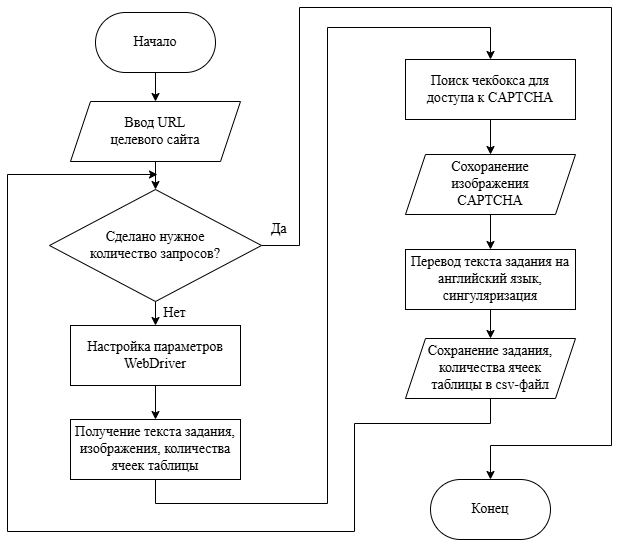
\includegraphics[width=0.65\textwidth]{imgs/image_captcha_flow.png}
    \caption{Блок-схема процесса парсинга CAPTCHA.}
    \label{fig:captcha-flow}
\end{figure}
\vspace{-0.5cm}

Полученные изображения и метаданные (включая текст задания и параметры сетки) используются для формирования обучающего датасета, пригодного для дообучения модели YOLOv8 в задачах классификации и сегментации объектов.

\section{Предварительная обработка изображений датасета}

После получения достаточного количества изображений для составления датасета необходимо провести их предварительную обработку и разметку. Это один из самыхважных этапов работы, поскольку от качества разметки напрямую зависит точность и эффективность последующей работы модели.

Для корректной работы модели YOLO требуется создать иерархическую структуру папок, в которой изображения и соответствующие метки будут разделены на тренировочную и валидационную выборки. Стандартная структура включает следующие директории:

\begin{enumerate}
    \item Директория train -- содержит тренировочную выборку:
    \begin{enumerate}
        \item images -- изображения;
        \item labels -- метки к изображениям.
    \end{enumerate}
    \item Директория val -- содержит валидационную выборку:
    \begin{enumerate}
        \item images -- изображения;
        \item labels -- метки к изображениям.
    \end{enumerate}
\end{enumerate}

Набор классов, пути к выборкам и параметры конфигурации задаются в YAML-файле, который передается при обучении модели. Содержимое такого файла для данной модели:

\begin{code}
\captionof{listing}{\label{code:train-captcha}Параметры конфигурации для обучения модели}
\vspace{-0.5cm}
{\small
\inputminted[mathescape,linenos,frame=lines,breaklines]{yaml}{code/train_captcha.yaml}
}
\end{code}
\vspace{-0.4cm}

Для создания меток используется инструмент CVAT (Computer Vision Annotation Tool) -- многофункциональное веб-приложение с поддержкой аннотации объектов с помощью полигонов, прямоугольников и других форм. CVAT позволяет экспортировать разметку напрямую в формат, совместимый с YOLO~\cite{CVAT}.

Поскольку CAPTCHA-изображения часто содержат объекты с нечёткими контурами, наложением и визуальными искажениями, особенно важно использовать ручную точную разметку, а не ограничиваться автоматическими методами. Выделение объектов должно проводиться как можно точнее, с учётом геометрии контуров. На рисунке ниже представлен пример изображения с размеченными объектами:

\begin{figure}[H]
    \centering
    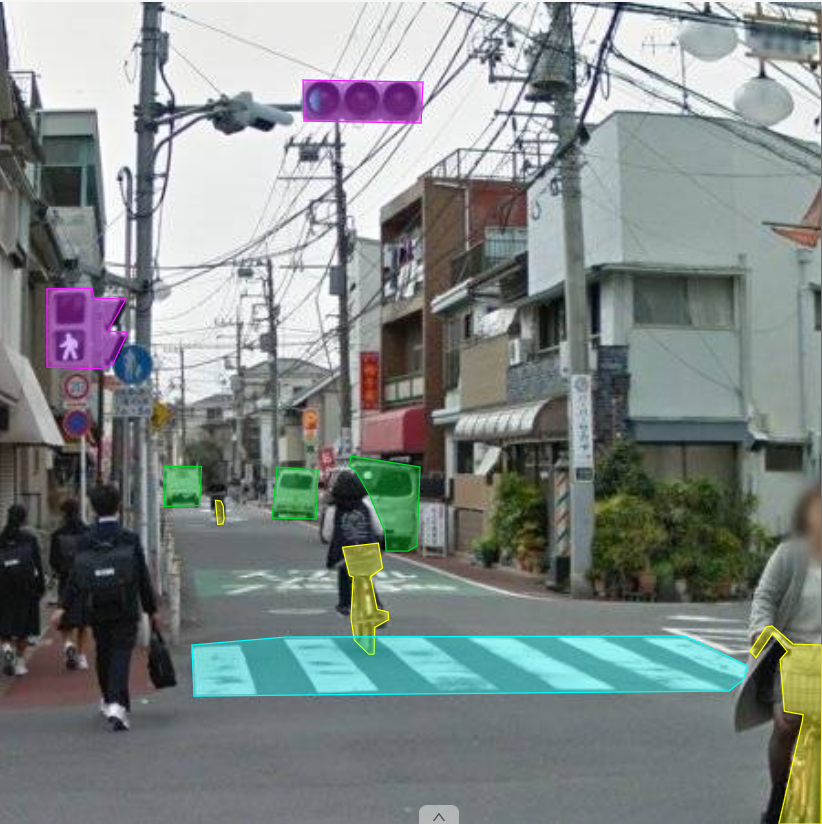
\includegraphics[width=0.9\linewidth]{imgs/captcha-poligons.png}
    \caption{Пример разметки изображения с тестовой CAPTCHA.}
    \label{fig:mask-captcha}
\end{figure}
\vspace{-0.5cm}

Кроме того, разметка позволяет учесть сразу несколько объектов разных классов на одном изображении, что особенно характерно для CAPTCHA, где в одной сетке могут одновременно находиться, например, автомобили и автобусы. Такой подход положительно влияет на обобщающую способность модели.

В случае, если количество данных по отдельным классам окажется недостаточным, можно дополнительно использовать методы аугментации: вращение, масштабирование, искажение цвета и контраста. Однако при хорошо организованном парсинге и разметке зачастую удается обойтись без аугментации.

% \input{chapter-3-csae}

\newpage
\addcontentsline{toc}{chapter}{СПИСОК ИСПОЛЬЗОВАННОЙ ЛИТЕРАТУРЫ}
\printbibliography[title={СПИСОК ИСПОЛЬЗОВАННОЙ ЛИТЕРАТУРЫ}]

\appendix
\newpage
\chapter*{\begin{flushright}\raggedleft\label{appendix1}Приложение 1\end{flushright}}
\phantomsection\addcontentsline{toc}{chapter}{ПРИЛОЖЕНИЕ 1}
\vspace{-1.75cm}

\begin{center}
\label{code:appendix}Текст программ для автоматизации решения аудио CAPTCHA
\end{center}

\begin{code}
    \captionof{listing}{\label{code:audiocaptcha}Исходный код расшифровки Audio CAPTCHA}
    \vspace{-1cm}
    \inputminted{python}{code/audiocaptcha/audiocaptcha.py}
\end{code}

\begin{code}
    \captionof{listing}{\label{code:audiocaptcha-solve}Исходный код автоматизированного решения Audio CAPTCHA}
    \vspace{-1cm}
    \inputminted{python}{code/audiocaptcha/audiocaptcha_solve.py}
\end{code}

\appendix
\newpage
\chapter*{\begin{flushright}\raggedleft\label{appendix2}Приложение 2\end{flushright}}
\phantomsection\addcontentsline{toc}{chapter}{ПРИЛОЖЕНИЕ 2}
\vspace{-1.75cm}

\begin{center}
\label{code:appendix2}Текст программ для автоматизации решения текстовых CAPTCHA
\end{center}

\begin{code}
    \captionof{listing}{\label{code:gen-dataset}Исходный код генератора синтетических текстовых CAPTCHA}
    \vspace{-1cm}
    \inputminted{python}{code/textcaptcha/gen-dataset.py}
\end{code}

\begin{code}
    \captionof{listing}{\label{code:preprocessing}Исходный код для предобработки изображений датасета с текстовыми CAPTCHA}
    \vspace{-1cm}
    \inputminted{python}{code/textcaptcha/preprocessing.py}
\end{code}

\begin{code}
    \captionof{listing}{\label{code:tf-dataset}Исходный код для создания датасета текстовых CAPTCHA в формате тензоров}
    \vspace{-1cm}
    \inputminted{python}{code/textcaptcha/tf-dataset.py}
\end{code}

\begin{code}
    \captionof{listing}{\label{code:crnn}Исходный код CRNN модели}
    \vspace{-1cm}
    \inputminted{python}{code/textcaptcha/crnn.py}
\end{code}

\begin{code}
    \captionof{listing}{\label{code:seq2seq}Исходный код Seq2Seq модели}
    \vspace{-1cm}
    \inputminted{python}{code/textcaptcha/seq-to-seq.py}
\end{code}

\begin{code}
    \captionof{listing}{\label{code:test-model}Исходный код тестирования Seq2Seq модели}
    \vspace{-1cm}
    \inputminted{python}{code/textcaptcha/test.py}
\end{code}

\appendix
\newpage
\chapter*{\begin{flushright}\raggedleft\label{appendix3}Приложение 3\end{flushright}}
\phantomsection\addcontentsline{toc}{chapter}{ПРИЛОЖЕНИЕ 3}
\vspace{-1.75cm}

\begin{center}
\label{code:appendix3}Текст программ для автоматизации решения графических CAPTCHA
\end{center}

\begin{code}
    \captionof{listing}{\label{code:get-captcha}Исходный код получения графических CAPTCHA с целевого сайта}
    \vspace{-1cm}
    \inputminted{python}{code/imagecaptcha/get_captcha.py}
\end{code}

\begin{code}
    \captionof{listing}{\label{code:recognize}Исходный код дообучения модели на датасете с графическими CAPTCHA}
    \vspace{-1cm}
    \inputminted{python}{code/imagecaptcha/recognize_objects.py}
\end{code}

\begin{code}
    \captionof{listing}{\label{code:solve-captcha}Исходный код автоматизированного решения графических CAPTCHA}
    \vspace{-1cm}
    \inputminted{python}{code/imagecaptcha/solve_captcha.py}
\end{code}

\makelastpage
\end{document}
